%LTeX: language=pt-br
% !TeX root = Apostila_IM381.tex

\cleardoublepage
\section{Elemento isoparamétrico}

    \subsection{Elemento quadrangular isoparamétrico}

        De forma geral, em um domínio de elementos finitos, pode haver vários elementos quadrangulares com formas diferentes ao longo do domínio. A ideia de definir um elemento isoparamétrico, é similar ao que fizemos no elemento de barra na Seção \ref{sec:elemento_barra}, queremos definir um único elemento em um sistema de coordenadas locais, com funções de forma definidas nessas coordenadas locais. Este elemento pode ser transformado e distorcido para encaixá-lo mesmo em geometrias que não sejam exatamente a dele. Evidentemente, quanto mais distorcido o elemento for, pior ele aproximará a resposta, e mais erros vamos inserir na solução. A próxima seção abordará este tema em mais detalhes.

        Considere então um elemento quadrangular qualquer em uma malha de elementos finitos no sistema de coordenadas globais $xy$. Este será transformado em um quadrado no sistema de coordenadas locais $\xi \eta$ (Figura \ref{fig:elemento_quadrado}).

        \begin{figure}[h!]
            \centering
            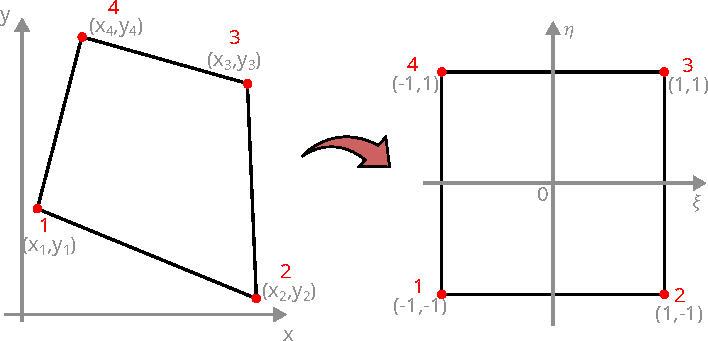
\includegraphics[scale=1]{Figures/9-Isoparametrico/Quadrado.pdf}
            \caption{Mapeamento entre um elemento quadrangular qualquer para um quadrado regular}
            \label{fig:elemento_quadrado}
        \end{figure}

        Para construir as funções de forma deste elemento, construímos funções de forma com polinômios de Lagrange (Seção \ref{sec:lagrange}):

        \begin{equation*}
            f_1(\xi) = \frac{1}{2}\left(1-\xi\right) \quad \quad f_1(\eta) = \frac{1}{2}\left(1-\eta\right)
        \end{equation*}

        \begin{equation*}
            f_2(\xi) = \frac{1}{2}\left(1+\xi\right) \quad \quad f_2(\eta) = \frac{1}{2}\left(1+\eta\right)
        \end{equation*}

        As funções de forma deste elemento são montadas multiplicando cada combinação dessas funções. Estas funções mantêm a propriedade dos polinômios de Lagrange de apenas uma ser unitária em cada nó e as outras serem nulas:

        \begin{equation}
            \begin{array}{l}
                N_1(\xi, \eta) = f_1(\xi)f_1(\eta) = \frac{1}{4}\left(1-\xi\right)\left(1-\eta\right)\\
                N_2(\xi, \eta) = f_2(\xi)f_1(\eta) = \frac{1}{4}\left(1+\xi\right)\left(1-\eta\right)\\
                N_3(\xi, \eta) = f_2(\xi)f_2(\eta) = \frac{1}{4}\left(1+\xi\right)\left(1+\eta\right)\\
                N_4(\xi, \eta) = f_1(\xi)f_2(\eta) = \frac{1}{4}\left(1-\xi\right)\left(1+\eta\right)\\
            \end{array}
        \end{equation}

        Ao definir as funções de forma de um elemento, é importante manter a consistência entre a numeração dos nós. No caso do elemento quadrado, numeramos os nós em sentido anti-horário (Figura \ref{fig:elemento_quadrado}). Finalmente, este elemento é normalmente dito como bilinear, visto que suas funções são lineares em cada variável $\xi$ e $\eta$, mas não são lineares, pois incluem o termo cruzado $\xi \eta$.

        As derivadas dessas funções de forma, em relação às coordenadas locais são:

        \begin{equation*}
            \frac{\partial N_1}{\partial \xi} = -\frac{1}{4}\left(1-\eta\right)  \quad \quad 
            \frac{\partial N_1}{\partial \eta} = -\frac{1}{4}\left(1-\xi\right)
        \end{equation*}

        \begin{equation*}
            \frac{\partial N_2}{\partial \xi} = \frac{1}{4}\left(1-\eta\right)  \quad \quad 
            \frac{\partial N_2}{\partial \eta} = -\frac{1}{4}\left(1+\xi\right)
        \end{equation*}

        \begin{equation*}
            \frac{\partial N_3}{\partial \xi} = \frac{1}{4}\left(1+\eta\right)  \quad \quad 
            \frac{\partial N_3}{\partial \eta} = \frac{1}{4}\left(1+\xi\right)
        \end{equation*}

        \begin{equation}
            \frac{\partial N_4}{\partial \xi} = -\frac{1}{4}\left(1+\eta\right)  \quad \quad 
            \frac{\partial N_4}{\partial \eta} = \frac{1}{4}\left(1-\xi\right)
        \end{equation}


        A relação entre as coordenadas locais e global é:

        \begin{equation*}
            x(\xi, \eta) = \sum N_i(\xi,\eta) x_i
        \end{equation*}

        \begin{equation}
            y(\xi, \eta) = \sum N_i(\xi,\eta) y_i
        \end{equation}

        As derivadas, em relação às coordenadas locais, são:

        \begin{equation*}
            \frac{\partial x}{\partial \xi} = \left(x_1-x_2+x_3-x_4\right)\eta + \left(-x_1+x_2+x_3-x_4\right)
        \end{equation*}

        \begin{equation*}
            \frac{\partial x}{\partial \eta} = \left(x_1-x_2+x_3-x_4\right)\xi + \left(-x_1-x_2+x_3+x_4\right)
        \end{equation*}

        \begin{equation*}
            \frac{\partial y}{\partial \xi} = \left(y_1-y_2+y_3-y_4\right)\eta + \left(-y_1+y_2+y_3-y_4\right)
        \end{equation*}

        \begin{equation*}
            \frac{\partial y}{\partial \eta} = \left(y_1-y_2+y_3-y_4\right)\xi + \left(-y_1-y_2+y_3+y_4\right)
        \end{equation*}

        Com isso, temos a matriz Jacobiana:

        \begin{equation}
            \mathbf{J}(\xi, \eta) = 
            \begin{bmatrix}
                 \frac{\partial x}{\partial \xi} &  \frac{\partial y}{\partial \xi}\\
                 \frac{\partial x}{\partial \eta} &  \frac{\partial y}{\partial \eta}
            \end{bmatrix}
        \end{equation}

        \noindent note que, neste caso, o Jacobiano não necessariamente será constante. Consequentemente, seu determinante também não será constante.

        As derivadas das funções de forma em relação às coordenadas globais são obtidas como na Seção \ref{sec:elemento_triangular}:

        \begin{equation}
            \begin{Bmatrix}
                \frac{\partial N_i}{\partial x} \\
                \frac{\partial N_i}{\partial y}
            \end{Bmatrix} = 
            \mathbf{J}^{-1}
            \begin{Bmatrix}
                \frac{\partial N_i}{\partial \xi} \\
                \frac{\partial N_i}{\partial \eta}
            \end{Bmatrix}
        \end{equation}

        Com as derivadas, podemos montar a matriz $\mathbf{B}$ do elemento. Por exemplo, no elemento de estado plano (Seção \ref{sec:estado_plano}):

        \begin{equation}
            \mathbf{B} = 
            \begin{bmatrix}
                \frac{\partial N_1}{\partial x} & 0 & \cdots & \frac{\partial N_n}{\partial x} & 0\\
                0 & \frac{\partial N_1}{\partial y} & \cdots & 0 & \frac{\partial N_n}{\partial y}\\
                \frac{\partial N_1}{\partial y} & \frac{\partial N_1}{\partial x} & \cdots & \frac{\partial N_n}{\partial y} & \frac{\partial N_n}{\partial x}\\
            \end{bmatrix}
        \end{equation}

        Com isso, podemos encontrar a matriz de rigidez de um elemento resolvendo a integral:

        \begin{equation}
            \mathbf{K}_e = \int_\Omega  \mathbf{B}^T \mathbf{D} \mathbf{B} dA
        \end{equation}

        Aplicando uma mudança de variáveis:

        \begin{equation}
            \mathbf{K}_e = \int_{-1}^{1} \int_{-1}^{1}  \mathbf{B}^T \mathbf{D} \mathbf{B} \det \mathbf{J} d\xi d\eta
        \end{equation}


    \subsection{Elemento hexaédrico isoparamétrico}

        Da mesma forma que a construção de um elemento quadrangular é feita pela multiplicação de funções de forma unidimensionais, para um elemento hexaédrico (Figura \ref{fig:elemento_cubo}), isto é feito de forma similar:

        \begin{figure}[h!]
            \centering
            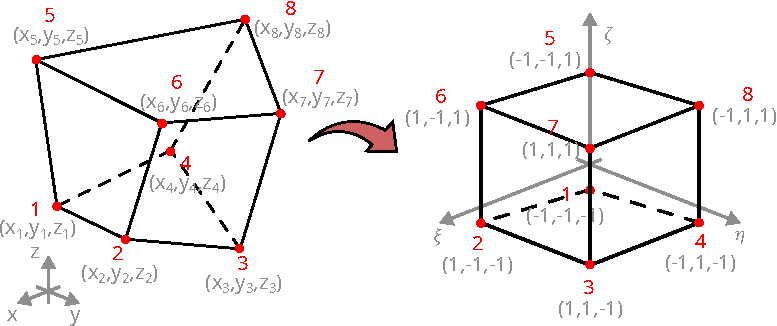
\includegraphics[scale=1]{Figures/9-Isoparametrico/Hexaedro.pdf}
            \caption{Mapeamento entre um elemento hexaédrico qualquer para um cubo regular}
            \label{fig:elemento_cubo}
        \end{figure}

        \begin{equation}
            \begin{array}{l}
                N_1(\xi, \eta, \zeta) = f_1(\xi)f_1(\eta)f_1(\zeta) = \frac{1}{8}\left(1-\xi\right)\left(1-\eta\right)\left(1-\zeta\right)\\
                N_2(\xi, \eta, \zeta) = f_2(\xi)f_1(\eta)f_1(\zeta) = \frac{1}{8}\left(1+\xi\right)\left(1-\eta\right)\left(1-\zeta\right)\\
                N_3(\xi, \eta, \zeta) = f_2(\xi)f_2(\eta)f_1(\zeta) = \frac{1}{8}\left(1+\xi\right)\left(1+\eta\right)\left(1-\zeta\right)\\
                N_4(\xi, \eta, \zeta) = f_1(\xi)f_2(\eta)f_1(\zeta) = \frac{1}{8}\left(1-\xi\right)\left(1+\eta\right)\left(1-\zeta\right)\\
                N_5(\xi, \eta, \zeta) = f_1(\xi)f_1(\eta)f_2(\zeta) = \frac{1}{8}\left(1-\xi\right)\left(1-\eta\right)\left(1+\zeta\right)\\
                N_6(\xi, \eta, \zeta) = f_2(\xi)f_1(\eta)f_2(\zeta) = \frac{1}{8}\left(1+\xi\right)\left(1-\eta\right)\left(1+\zeta\right)\\
                N_7(\xi, \eta, \zeta) = f_2(\xi)f_2(\eta)f_2(\zeta) = \frac{1}{8}\left(1+\xi\right)\left(1+\eta\right)\left(1+\zeta\right)\\
                N_8(\xi, \eta, \zeta) = f_1(\xi)f_2(\eta)f_2(\zeta) = \frac{1}{8}\left(1-\xi\right)\left(1+\eta\right)\left(1+\zeta\right)\\
            \end{array}
        \end{equation}
    
        Suas derivadas são:

        \begin{equation*}
            \frac{\partial N_1}{\partial \xi} = -\frac{1}{8}\left(1-\eta\right)\left(1-\zeta\right)  \quad \quad 
            \frac{\partial N_1}{\partial \eta} = -\frac{1}{8}\left(1-\xi\right)\left(1-\zeta\right)  \quad \quad 
            \frac{\partial N_1}{\partial \zeta} = -\frac{1}{8}\left(1-\xi\right)\left(1-\eta\right)
        \end{equation*}

        \begin{equation*}
            \frac{\partial N_2}{\partial \xi} =  \frac{1}{8}\left(1-\eta\right)\left(1-\zeta\right)  \quad \quad 
            \frac{\partial N_2}{\partial \eta} = -\frac{1}{8}\left(1+\xi\right)\left(1-\zeta\right)  \quad \quad 
            \frac{\partial N_2}{\partial \zeta} = -\frac{1}{8}\left(1+\xi\right)\left(1-\eta\right)
        \end{equation*}

        \begin{equation*}
            \frac{\partial N_3}{\partial \xi} =  \frac{1}{8}\left(1+\eta\right)\left(1-\zeta\right)  \quad \quad 
            \frac{\partial N_3}{\partial \eta} =  \frac{1}{8}\left(1+\xi\right)\left(1-\zeta\right)  \quad \quad 
            \frac{\partial N_3}{\partial \zeta} = -\frac{1}{8}\left(1+\xi\right)\left(1+\eta\right)
        \end{equation*}

        \begin{equation*}
            \frac{\partial N_4}{\partial \xi} = -\frac{1}{8}\left(1+\eta\right)\left(1-\zeta\right)  \quad \quad 
            \frac{\partial N_4}{\partial \eta} =  \frac{1}{8}\left(1-\xi\right)\left(1-\zeta\right)  \quad \quad 
            \frac{\partial N_4}{\partial \zeta} = -\frac{1}{8}\left(1-\xi\right)\left(1+\eta\right)
        \end{equation*}

        \begin{equation*}
            \frac{\partial N_5}{\partial \xi} = -\frac{1}{8}\left(1-\eta\right)\left(1+\zeta\right)  \quad \quad 
            \frac{\partial N_5}{\partial \eta} = -\frac{1}{8}\left(1-\xi\right)\left(1+\zeta\right)  \quad \quad 
            \frac{\partial N_5}{\partial \zeta} =  \frac{1}{8}\left(1-\xi\right)\left(1-\eta\right)
        \end{equation*}

        \begin{equation*}
            \frac{\partial N_6}{\partial \xi} =  \frac{1}{8}\left(1-\eta\right)\left(1+\zeta\right)  \quad \quad 
            \frac{\partial N_6}{\partial \eta} = -\frac{1}{8}\left(1+\xi\right)\left(1+\zeta\right)  \quad \quad 
            \frac{\partial N_6}{\partial \zeta} =  \frac{1}{8}\left(1+\xi\right)\left(1-\eta\right)
        \end{equation*}

        \begin{equation*}
            \frac{\partial N_7}{\partial \xi} =  \frac{1}{8}\left(1+\eta\right)\left(1+\zeta\right)  \quad \quad 
            \frac{\partial N_7}{\partial \eta} =  \frac{1}{8}\left(1+\xi\right)\left(1+\zeta\right)  \quad \quad 
            \frac{\partial N_7}{\partial \zeta} =  \frac{1}{8}\left(1+\xi\right)\left(1+\eta\right)
        \end{equation*}

        \begin{equation}
            \frac{\partial N_8}{\partial \xi} = -\frac{1}{8}\left(1+\eta\right)\left(1+\zeta\right)  \quad \quad 
            \frac{\partial N_8}{\partial \eta} =  \frac{1}{8}\left(1-\xi\right)\left(1+\zeta\right)  \quad \quad 
            \frac{\partial N_8}{\partial \zeta} =  \frac{1}{8}\left(1-\xi\right)\left(1+\eta\right)
        \end{equation}

        A relação entre as coordenadas locais e global é:

        \begin{equation*}
            x(\xi, \eta, \zeta) = \sum N_i(\xi,\eta, \zeta) x_i
        \end{equation*}

        \begin{equation*}
            y(\xi, \eta, \zeta) = \sum N_i(\xi,\eta,\zeta) y_i
        \end{equation*}

        \begin{equation}
            z(\xi, \eta, \zeta) = \sum N_i(\xi,\eta,\zeta) z_i
        \end{equation}


        Com as derivadas das coordenadas em relação as coordenadas locais, temos a matriz Jacobiana:

        \begin{equation}
            \mathbf{J}(\xi, \eta, \zeta) = 
            \begin{bmatrix}
                \frac{\partial x}{\partial \xi} &  \frac{\partial y}{\partial \xi} &  \frac{\partial z}{\partial \xi}\\
                \frac{\partial x}{\partial \eta} &  \frac{\partial y}{\partial \eta} &  \frac{\partial z}{\partial \eta}\\
                \frac{\partial x}{\partial \zeta} &  \frac{\partial y}{\partial \zeta} &  \frac{\partial z}{\partial \zeta}
            \end{bmatrix}
        \end{equation}

        \noindent novamente, o Jacobiano não será constante. Consequentemente, seu determinante também não será constante.


        As derivadas das funções de forma em relação às coordenadas globais são obtidas como anteriormente:

        \begin{equation}
            \begin{Bmatrix}
                \frac{\partial N_i}{\partial x} \\
                \frac{\partial N_i}{\partial y} \\
                \frac{\partial N_i}{\partial z}
            \end{Bmatrix} = 
            \mathbf{J}^{-1}
            \begin{Bmatrix}
                \frac{\partial N_i}{\partial \xi} \\
                \frac{\partial N_i}{\partial \eta} \\
                \frac{\partial N_i}{\partial \zeta}
            \end{Bmatrix}
        \end{equation}

        Com as derivadas, podemos montar a matriz $\mathbf{B}$ do elemento. Nesta apostila, não será feita a dedução para o caso de elasticidade geral, mas ela é similar ao da Seção \ref{sec:estado_plano}:

        \begin{equation}
            \mathbf{B} = 
            \begin{bmatrix}
                \frac{\partial N_1}{\partial x} & 0 & 0 & \cdots & \frac{\partial N_n}{\partial x} & 0 & 0\\
                0 & \frac{\partial N_1}{\partial y} & 0 & \cdots & 0 & \frac{\partial N_n}{\partial y} & 0\\
                0 & 0 & \frac{\partial N_1}{\partial z} & \cdots & 0 & 0 & \frac{\partial N_n}{\partial z} \\
                \frac{\partial N_1}{\partial y} & \frac{\partial N_1}{\partial x} & 0 & \cdots & \frac{\partial N_n}{\partial y} & \frac{\partial N_n}{\partial x} & 0\\
                \frac{\partial N_1}{\partial z} & 0 & \frac{\partial N_1}{\partial x} & \cdots & \frac{\partial N_n}{\partial z} & 0 & \frac{\partial N_n}{\partial x}\\
                0 & \frac{\partial N_1}{\partial z} & \frac{\partial N_1}{\partial y} & \cdots & 0 & \frac{\partial N_n}{\partial z} & \frac{\partial N_n}{\partial y}\\
            \end{bmatrix}
        \end{equation}

        Para um material linear elástico isotrópico, temos a matriz constitutiva também:

        \begin{equation}
            \mathbf{D} =
            \frac{E}{\left(1+\nu\right)\left(1-2\nu\right)}
            \begin{bmatrix}
                1-\nu & \nu & \nu & 0 & 0 & 0\\
                \nu & 1-\nu & \nu & 0 & 0 & 0\\
                \nu & \nu & 1-\nu & 0 & 0 & 0\\
                0 & 0 & 0 & \frac{1-2\nu}{2} & 0 & 0\\
                0 & 0 & 0 & 0 & \frac{1-2\nu}{2} & 0\\
                0 & 0 & 0 & 0 & 0 & \frac{1-2\nu}{2}
            \end{bmatrix}
        \end{equation}

        Com isso, podemos encontrar a matriz de rigidez de um elemento resolvendo a integral:

        \begin{equation}
            \mathbf{K}_e = \int_\Omega  \mathbf{B}^T \mathbf{D} \mathbf{B} dV
        \end{equation}

        Aplicando uma mudança de variáveis:

        \begin{equation}
            \mathbf{K}_e = \int_{-1}^{1} \int_{-1}^{1} \int_{-1}^{1}  \mathbf{B}^T \mathbf{D} \mathbf{B} \det \mathbf{J} d\xi d\eta d\zeta
        \end{equation}



    \subsection{Integração no domínio 2D e 3D}
    \label{sec:integracaonD}

        Para integrar as matrizes dos elementos quadrangulares e hexaédricos, será utilizado o procedimento de integração por quadratura de Gauss-Legendre, conforme apresentado na Seção \ref{sec:integracao1D}.

        Considere uma função de duas ou de três variáveis, que devem ser integradas entre os limites $-1$ e $1$ para cada uma dessas. A integral será aproximada por:

        \begin{equation*}
            \int_{-1}^{1} \int_{-1}^{1} f(\xi, \eta) d\xi d\eta \approx 
            \sum\limits_{p=1}^{n_p} f(\xi_p,\eta_p) w_p = 
            \sum\limits_{i=1}^{n_1} \sum\limits_{j=1}^{n_2} f(\xi_i,\eta_j) w_i^{(\xi)} w_j^{(\eta)}
        \end{equation*}

        \begin{equation*}
            \int_{-1}^{1} \int_{-1}^{1} \int_{-1}^{1} f(\xi, \eta, \zeta) d\xi d\eta d\zeta \approx 
            \sum\limits_{p=1}^{n_p} f(\xi_p,\eta_p, \zeta_p) w_p = 
            \sum\limits_{i=1}^{n_1} \sum\limits_{j=1}^{n_2} \sum\limits_{k=1}^{n_3} f(\xi_i,\eta_j, \zeta_k) w_i^{(\xi)} w_j^{(\eta)} w_k^{(\zeta)}
        \end{equation*}

        Para encontrar os pontos de integração e os pesos, podemos considerar variável a variável. Isto é, consideramos apenas o procedimento de integração para uma função de uma variável $\xi$. Determinamos os pontos de integração e pesos $\xi_i, w_i^{(\xi)}$, baseado no grau do polinômio integrado em $\xi$. Em seguida, fazemos o mesmo para $\eta$ e $\zeta$. Finalmente, fazemos uma combinação dos pontos obtidos para cada variável (Figura \ref{fig:integracao_2d}). Portanto, se temos, por exemplo, em um caso 2D, 2 pontos para $\xi$ e 2 para $\eta$, teremos, no final, 4 pontos de integração.

        \begin{figure}[h!]
            \centering
            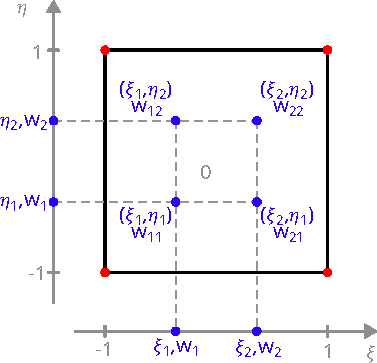
\includegraphics[scale=1.5]{Figures/9-Isoparametrico/Integracao.pdf}
            \caption{Integração em dimensões maiores a partir de uma dimensão}
            \label{fig:integracao_2d}
        \end{figure}

        Para elementos triangulares ou tetraédricos, o procedimento para obter os pontos de integração não é tão simples, visto que as integrais não têm limites constantes. Para este tipo de elemento, com funções de forma lineares, os termos da matriz de rigidez ficam constantes. Portanto, não é necessária uma integração numérica. Entretanto, se aumentamos a ordem dos elementos, ela se torna necessária; ou se integrarmos uma força mais complexa. Existem propostas para obter os pontos de integração desses elementos; entretanto, na prática, são usadas tabelas com os pontos de integração.

        \subsubsection{Exemplo}

        Resolva a integral abaixo usando integração de Gauss-Legendre:

        \begin{equation*}
            \int_{0}^{2} \int_{0}^{1} \left(x^2y + xy^2  \right) dx dy
        \end{equation*}

        \subsubsection*{Solução}

        A integral analítica pode ser obtida como:

        \begin{equation*}
            \int_{0}^{2} \int_{0}^{1} (x^2y + xy^2) dx dy = 
            \int_{0}^{2} \left[\frac{x^3}{3}y + \frac{x^2}{2}y^2\right]_0^1 dy
        \end{equation*}

        \begin{equation*}
            \int_{0}^{2} \frac{y}{3} + \frac{y^2}{2} dy = 
            \left[\frac{y^2}{6} + \frac{y^3}{6}\right]_0^2 = \frac{4}{6} + \frac{8}{6} = 2
        \end{equation*}

        Para integrar numericamente, precisamos fazer um mapeamento entre as coordenadas $x$ e $y$ para coordenadas locais $\xi$ e $\eta$, cujos limites de integração são $-1$ e $1$. No caso, $x$ apenas depende de $\xi$, e $y$, apenas de $\eta$:

        \begin{equation*}
            x(\xi) = \frac{1}{2}(1+\xi)
        \end{equation*}

        \begin{equation*}
            y(\eta) = 1+\eta
        \end{equation*}

        \begin{equation*}
            \frac{dx}{d\xi} = \frac{1}{2}
        \end{equation*}

        \begin{equation*}
            \frac{dy}{d\eta} = 1
        \end{equation*}

        O Jacobiano e seu determinante são:

        \begin{equation*}
            \mathbf{J} = 
            \begin{bmatrix}
                 \frac{\partial x}{\partial \xi} &  \frac{\partial y}{\partial \xi}\\
                 \frac{\partial x}{\partial \eta} &  \frac{\partial y}{\partial \eta}
            \end{bmatrix} =
            \begin{bmatrix}
                \frac{1}{2} & 0\\
                0 & 1
            \end{bmatrix}
        \end{equation*}

        \begin{equation*}
            \det \mathbf{J} = 
            \frac{1}{2}
        \end{equation*}

        \begin{equation*}
            \int_{0}^{2} \int_{0}^{1} (x^2y + xy^2) dx dy = 
            \int_{-1}^{1} \int_{-1}^{1} (x(\xi)^2y(\eta) + x(\xi)y(\eta)^2) \det \mathbf{J} d\xi d\eta 
        \end{equation*}

        Como são funções polinomiais em $\xi$ e $\eta$, podemos encontrar um número mínimo de pontos de Gauss tal que a integração seja exata:

        \begin{equation*}
            N_\xi \geq \frac{P_\xi+1}{2} = \frac{2+1}{2} = 1,5
        \end{equation*}

        \begin{equation*}
            N_\eta \geq \frac{P_\xi+1}{2} = \frac{2+1}{2} = 1,5
        \end{equation*}

        Finalmente, calculamos a integral para dois números de pontos de Gauss para verificar:

        \begin{equation*}
            n_x \times n_y =  1 \times 1 \rightarrow \int_{0}^{2} \int_{0}^{1} (x^2y + xy^2) dx dy \approx  1,5\rightarrow \text{erro de } 25\% 
        \end{equation*}

        \begin{equation*}
            n_x \times n_y =  2 \times 2 \rightarrow \int_{0}^{2} \int_{0}^{1} (x^2y + xy^2) dx dy =  2 \rightarrow \text{erro de } 0\% 
        \end{equation*}
